\documentclass{exam}
\usepackage[utf8]{inputenc}
\usepackage{graphicx}
\usepackage{amsmath}
\usepackage{tikz}
\usepackage{pgfplots}
\pgfplotsset{compat=1.11}
\usepackage[margin=2cm]{geometry}
\begin{document}
\makebox[\dimexpr\textwidth][r]{
\includegraphics[height=1.5cm]{./images/marca-udesc.png}} 
\makebox[\textwidth][l]{Nome: \enspace\hrulefill}
\makebox[\textwidth][l]{Turma: 1º F}
\makebox[\textwidth][l]{Professor: Mateus Schroeder da Silva}

\begin{questions}
    \question Seja $f(x) = 2^{x+1}$. 
    \begin{parts}
        \part[2] Encontre a função inversa. \\
        $2^{x+1} = y$ \\
        $\log 2^{x+1} = \log y$, log é uma função, então aplicar o log em ambos os lados mantém a igualdade \\
        $(x+1) \log 2 = \log y$, propriedade $ \log x^k = k \cdot \log x$ \\
        $x+1 = \dfrac{\log y}{\log 2}$, dividir ambos os lados por $\log 2$ \\
        $x = \dfrac{\log y}{\log 2} -1$, subtrair ambos os lados por $1$ \\
        $x = \log_2 y -1$, outra resposta possível, usando a propriedade $\frac{\log a}{\log b} = \log_b a$\\

        \part[2] Esboce o gráfico de ambas usando o plano representado logo abaixo (Dica: simetria).\\
        %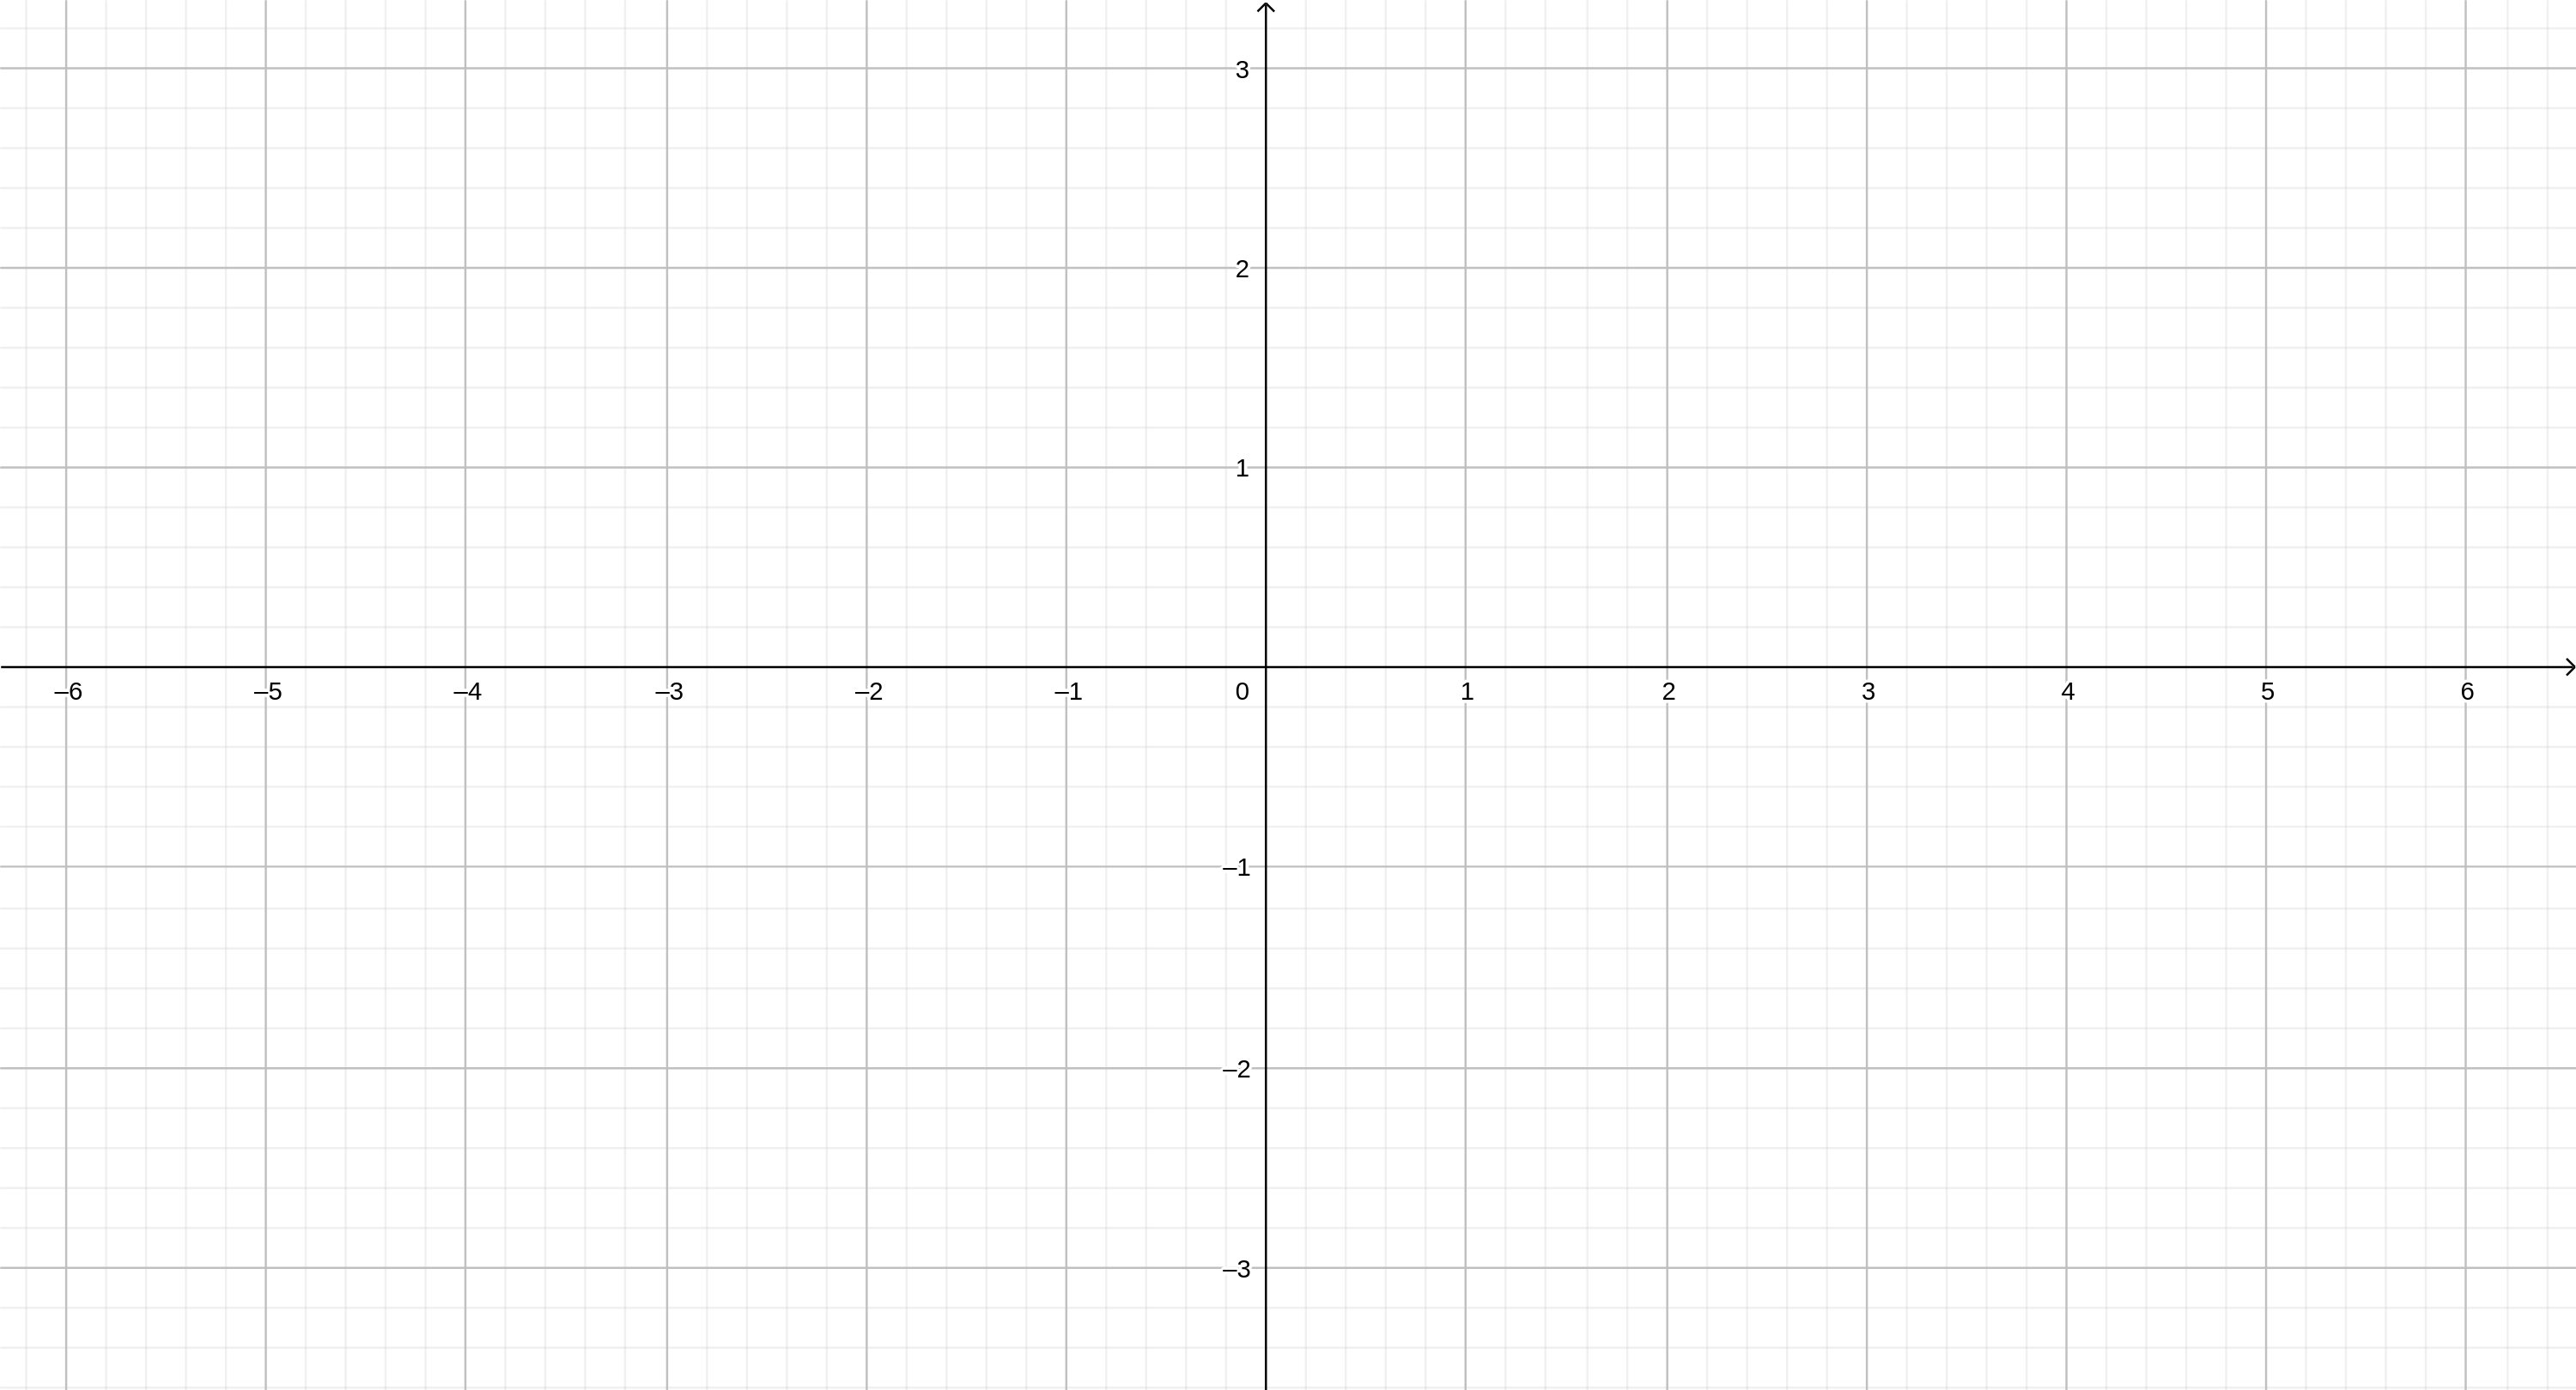
\includegraphics[height=4cm]{./images/Q1-pergunta.png}
        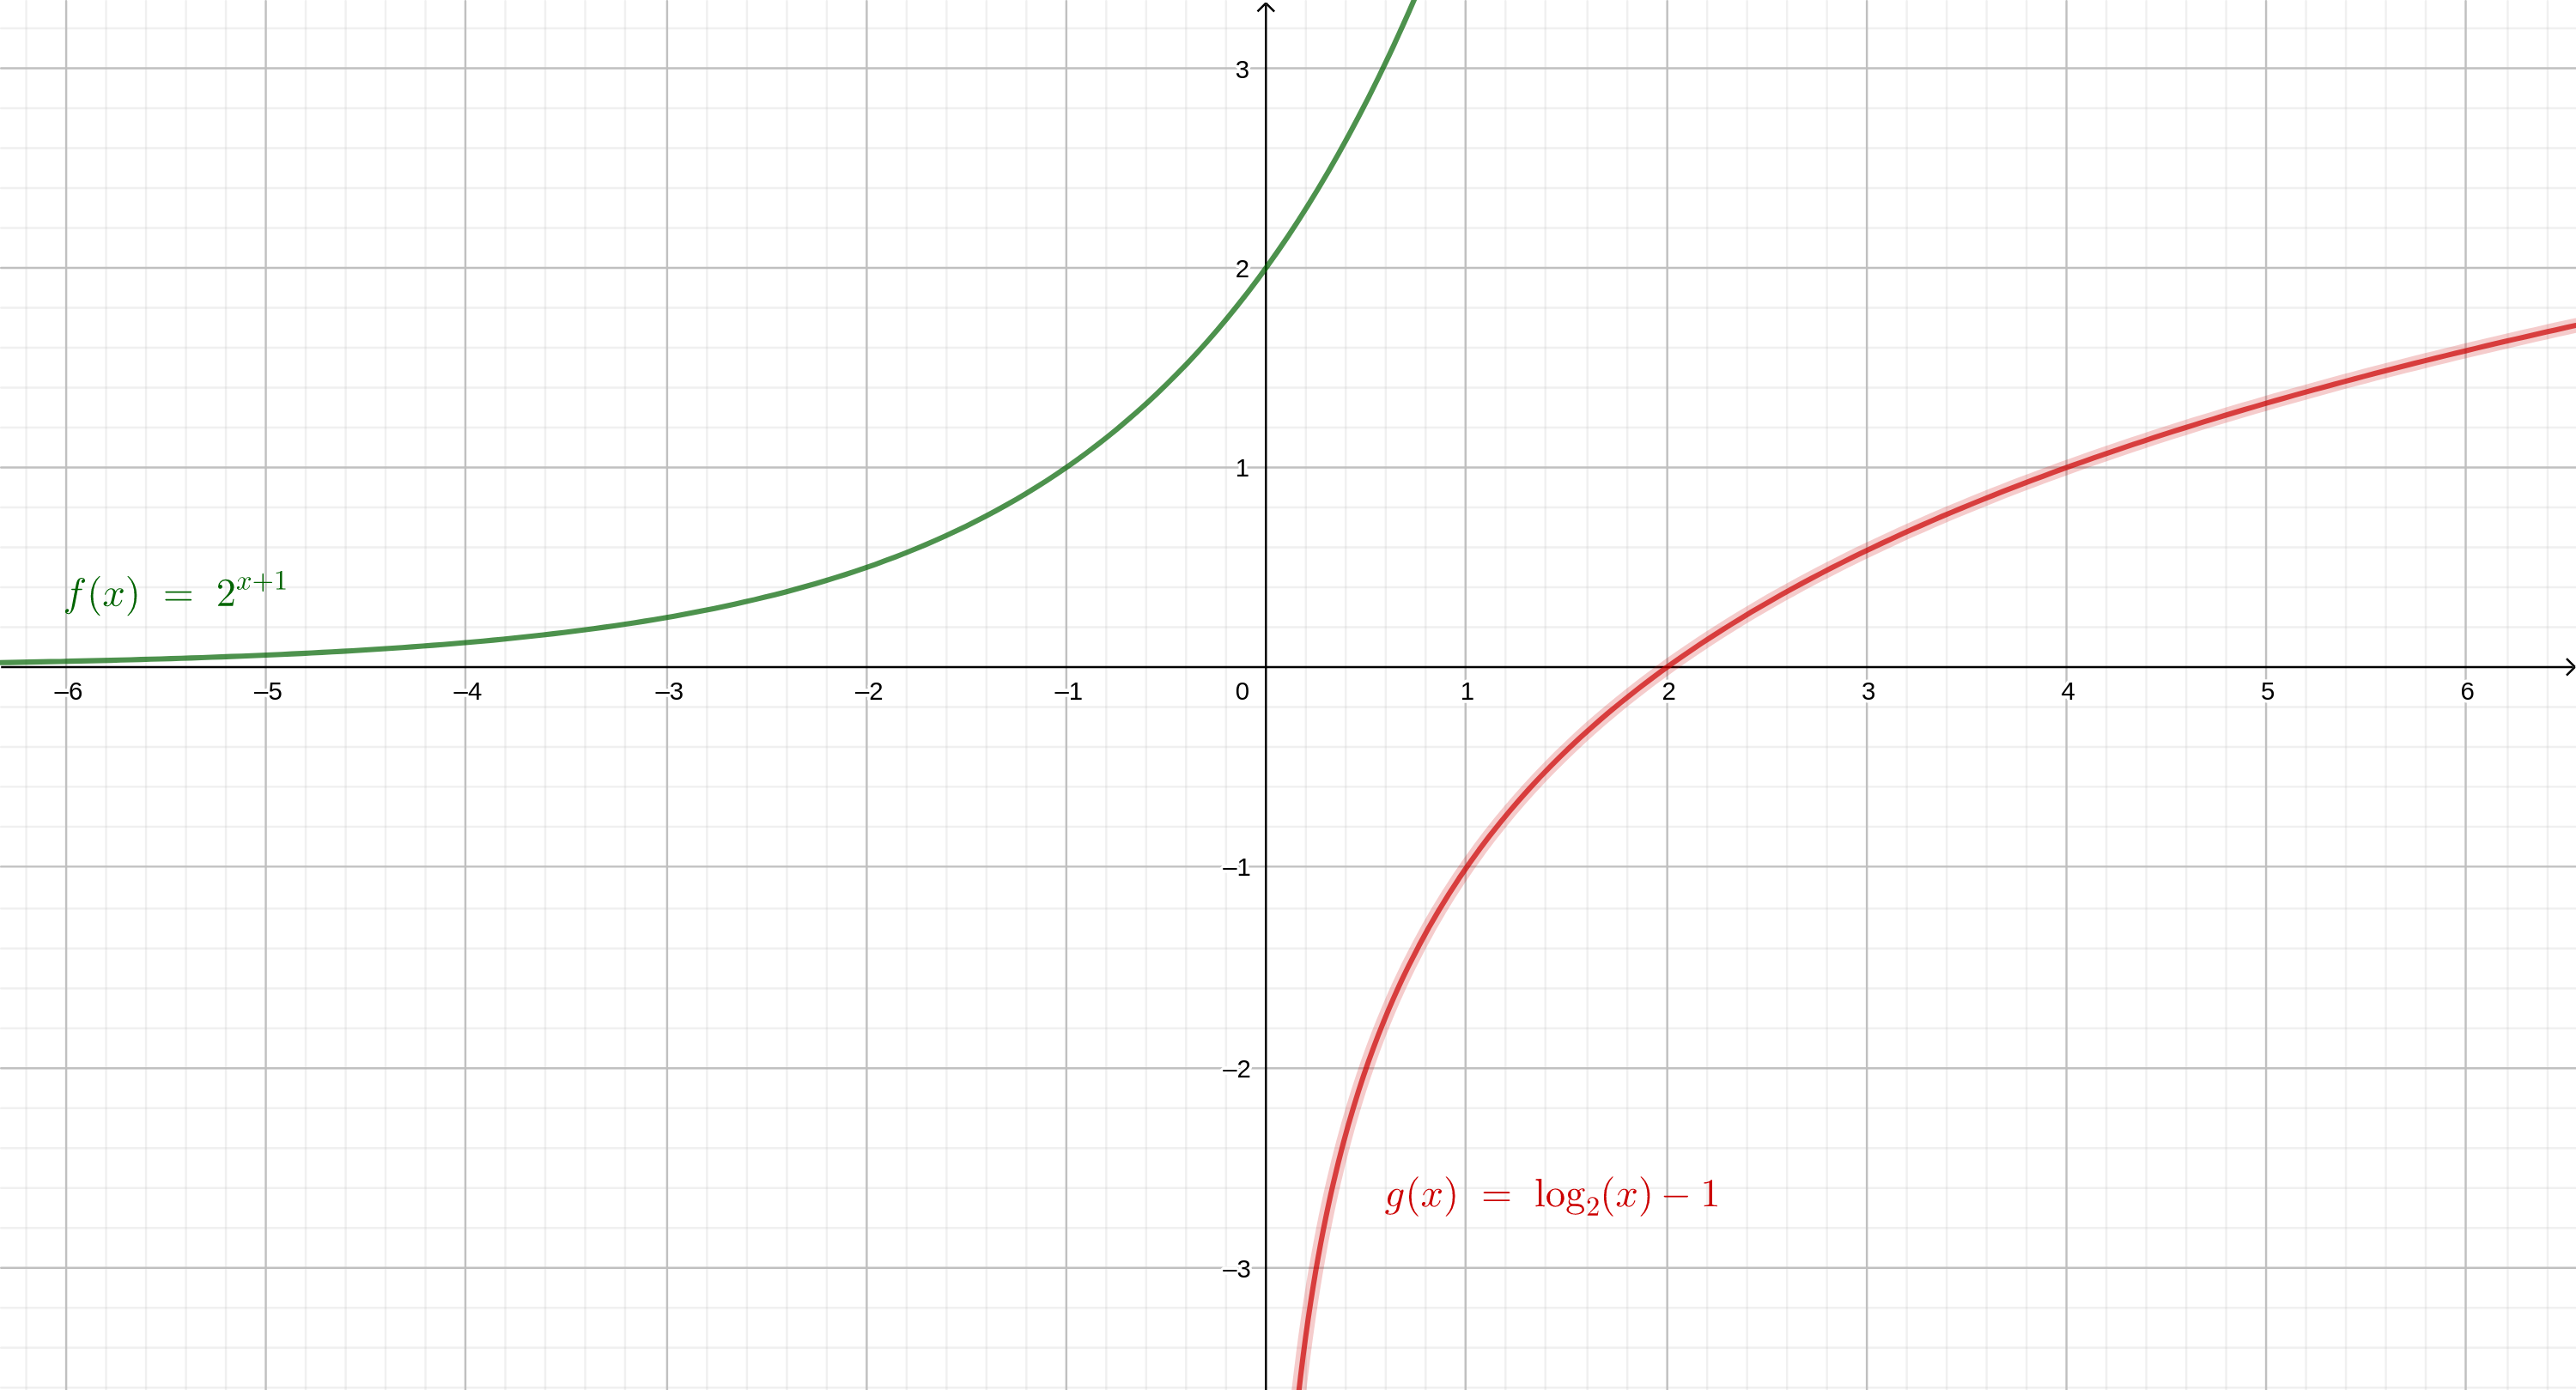
\includegraphics[height=4cm]{./images/Q1-resposta.png}
    \end{parts}

    \question Considere um título LCI (Letra de Crédito Imobiliário) de renda fixa de $10\%$ a.a. \\
    \begin{parts}
      \part[1]  Calcule quanto é o montante de uma aplicação de $R\$ 1000$ em cada ano, durante $5$ anos. \\
      Após 1 ano : $1000 \cdot 1,1^1 = 1000 \cdot 1,1 = R\$ 1.100,00$ \\
      Após 2 anos: $1000 \cdot 1,1^2 = 1000 \cdot 1,21 = R\$ 1.210,00$ \\
      Após 3 anos: $1000 \cdot 1,1^3 = 1000 \cdot 1,331 = R\$ 1.331,00$ \\
      Após 4 anos: $1000 \cdot 1,1^4 = 1000 \cdot 1,4641 = R\$ 1.464,10$ \\
      Após 5 anos: $1000 \cdot 1,1^5 = 1000 \cdot 1,61051 = R\$ 1.610,51$ 
      \part[1]  Esboce o gráfico do montante desta aplicação usando o plano representado logo abaixo. \\
        %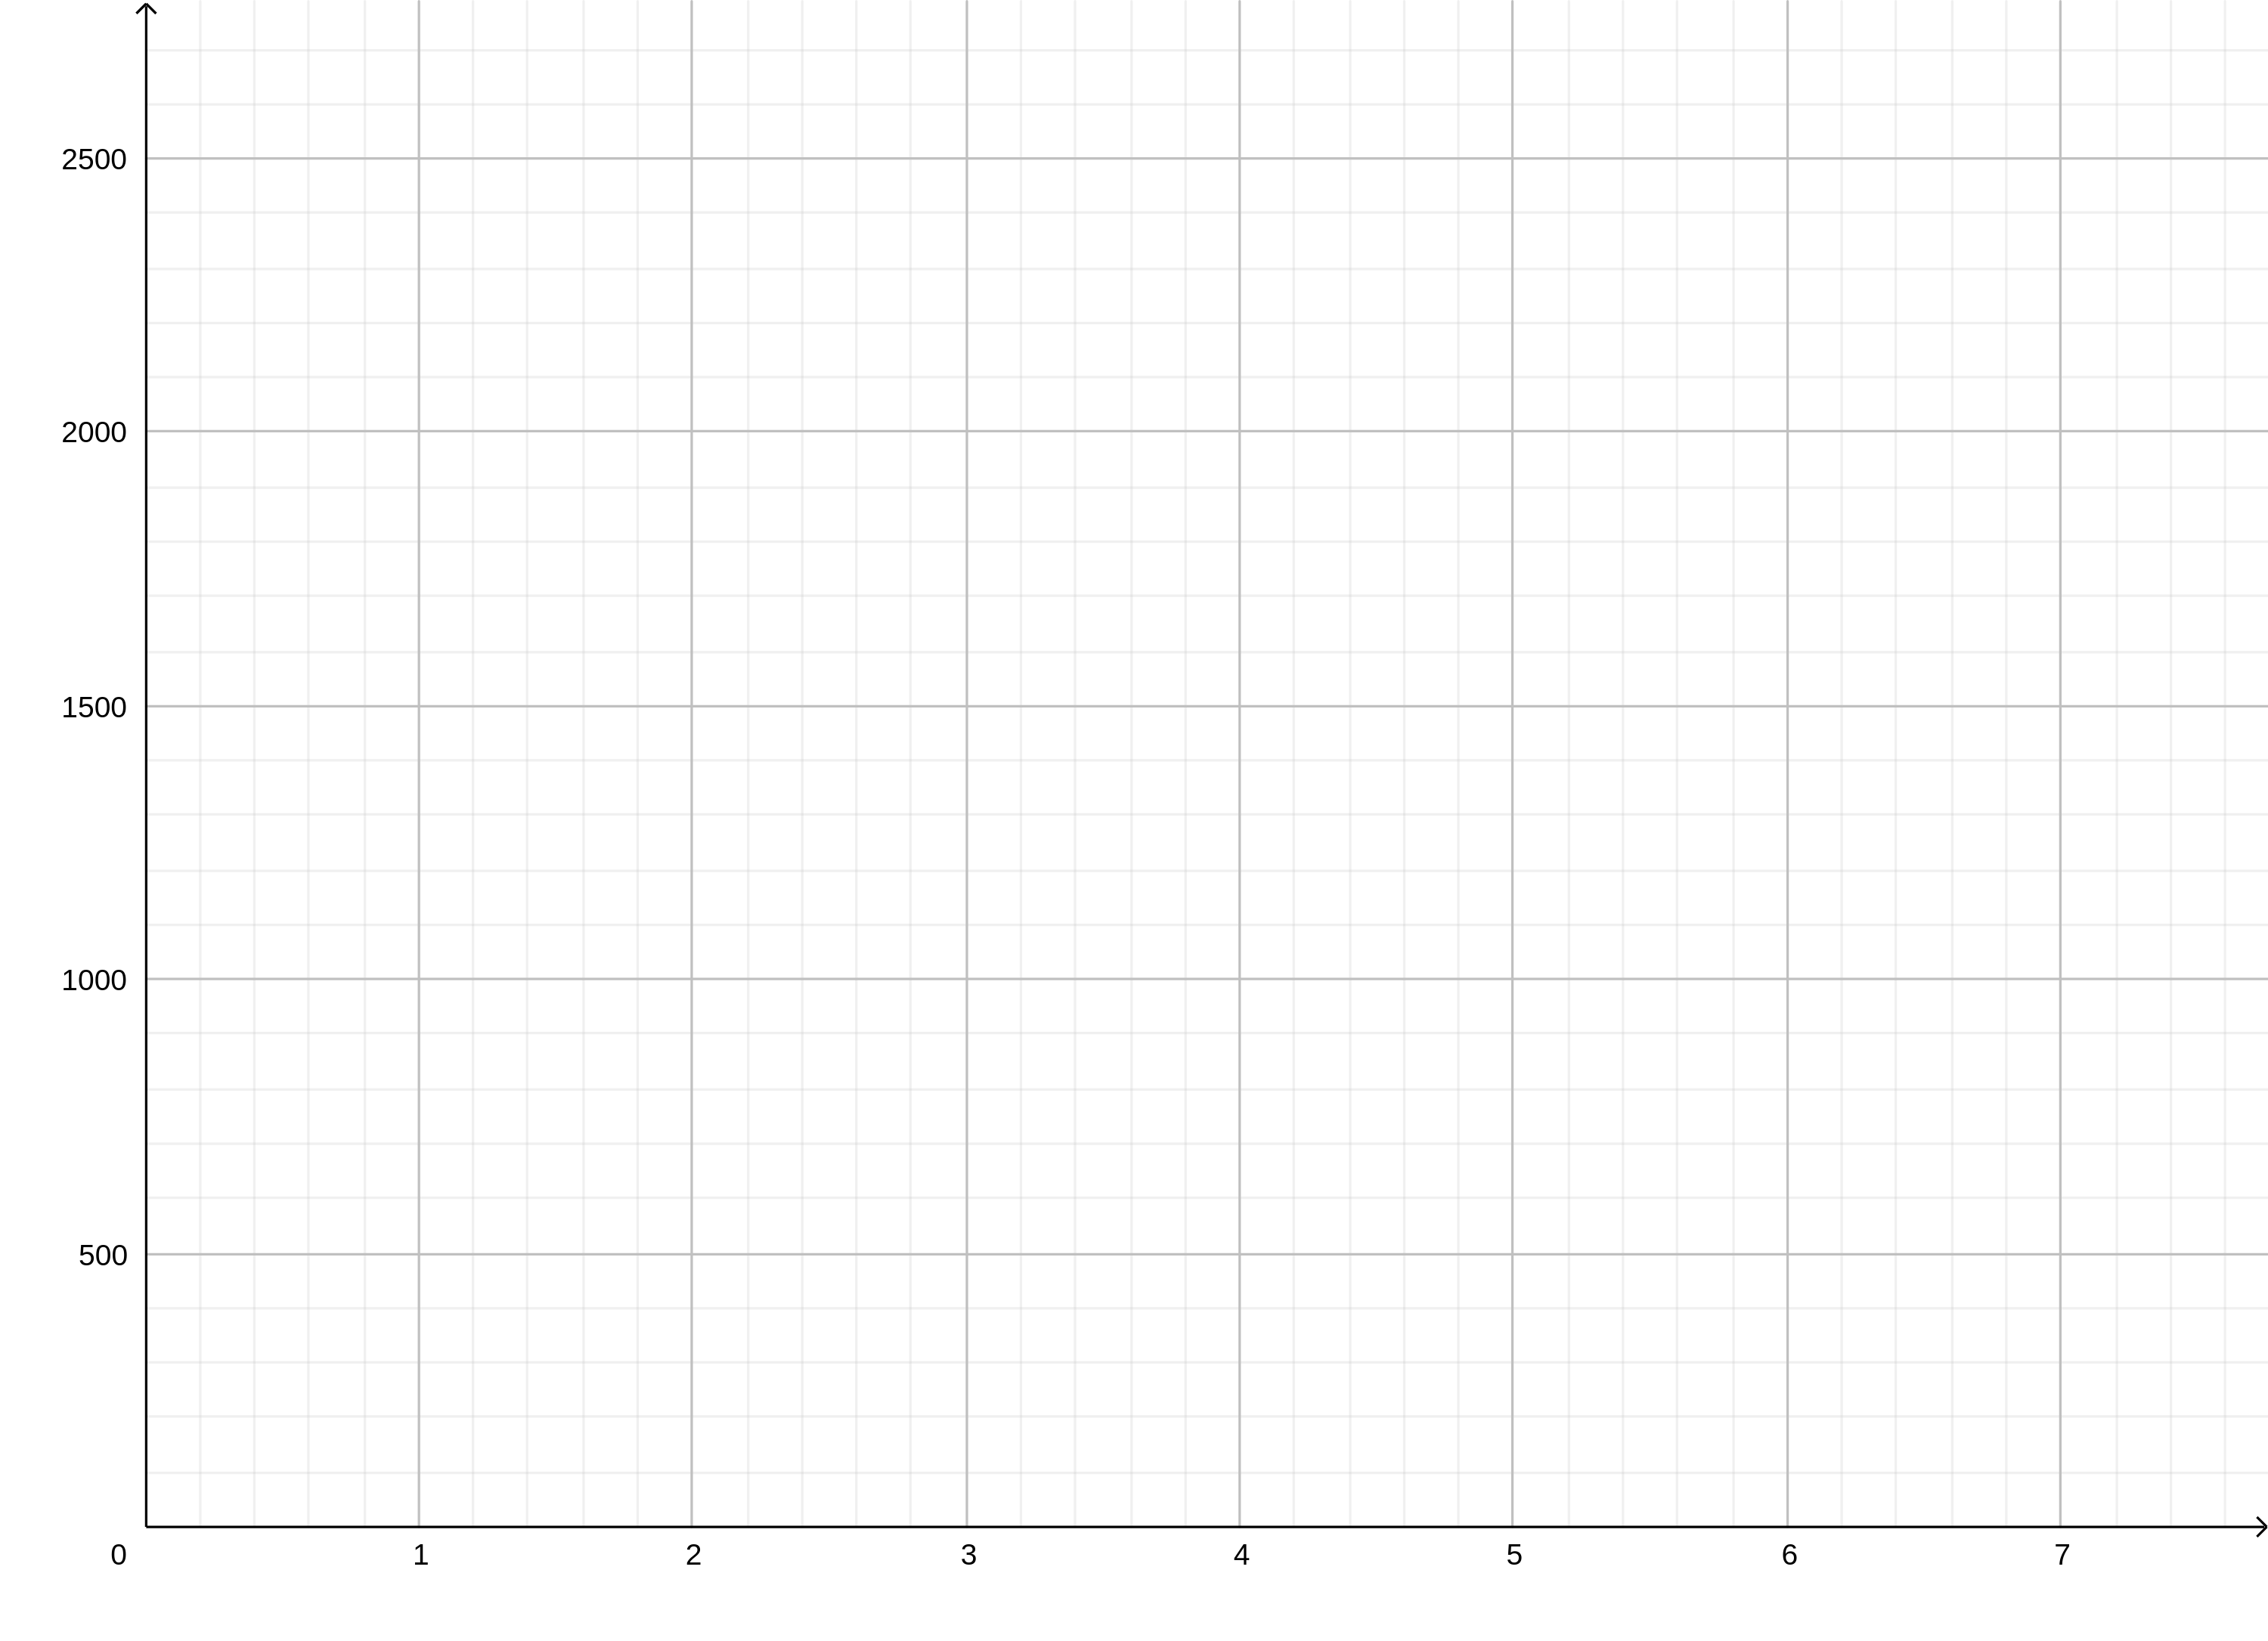
\includegraphics[height=4cm]{./images/Q2-pergunta.png}
        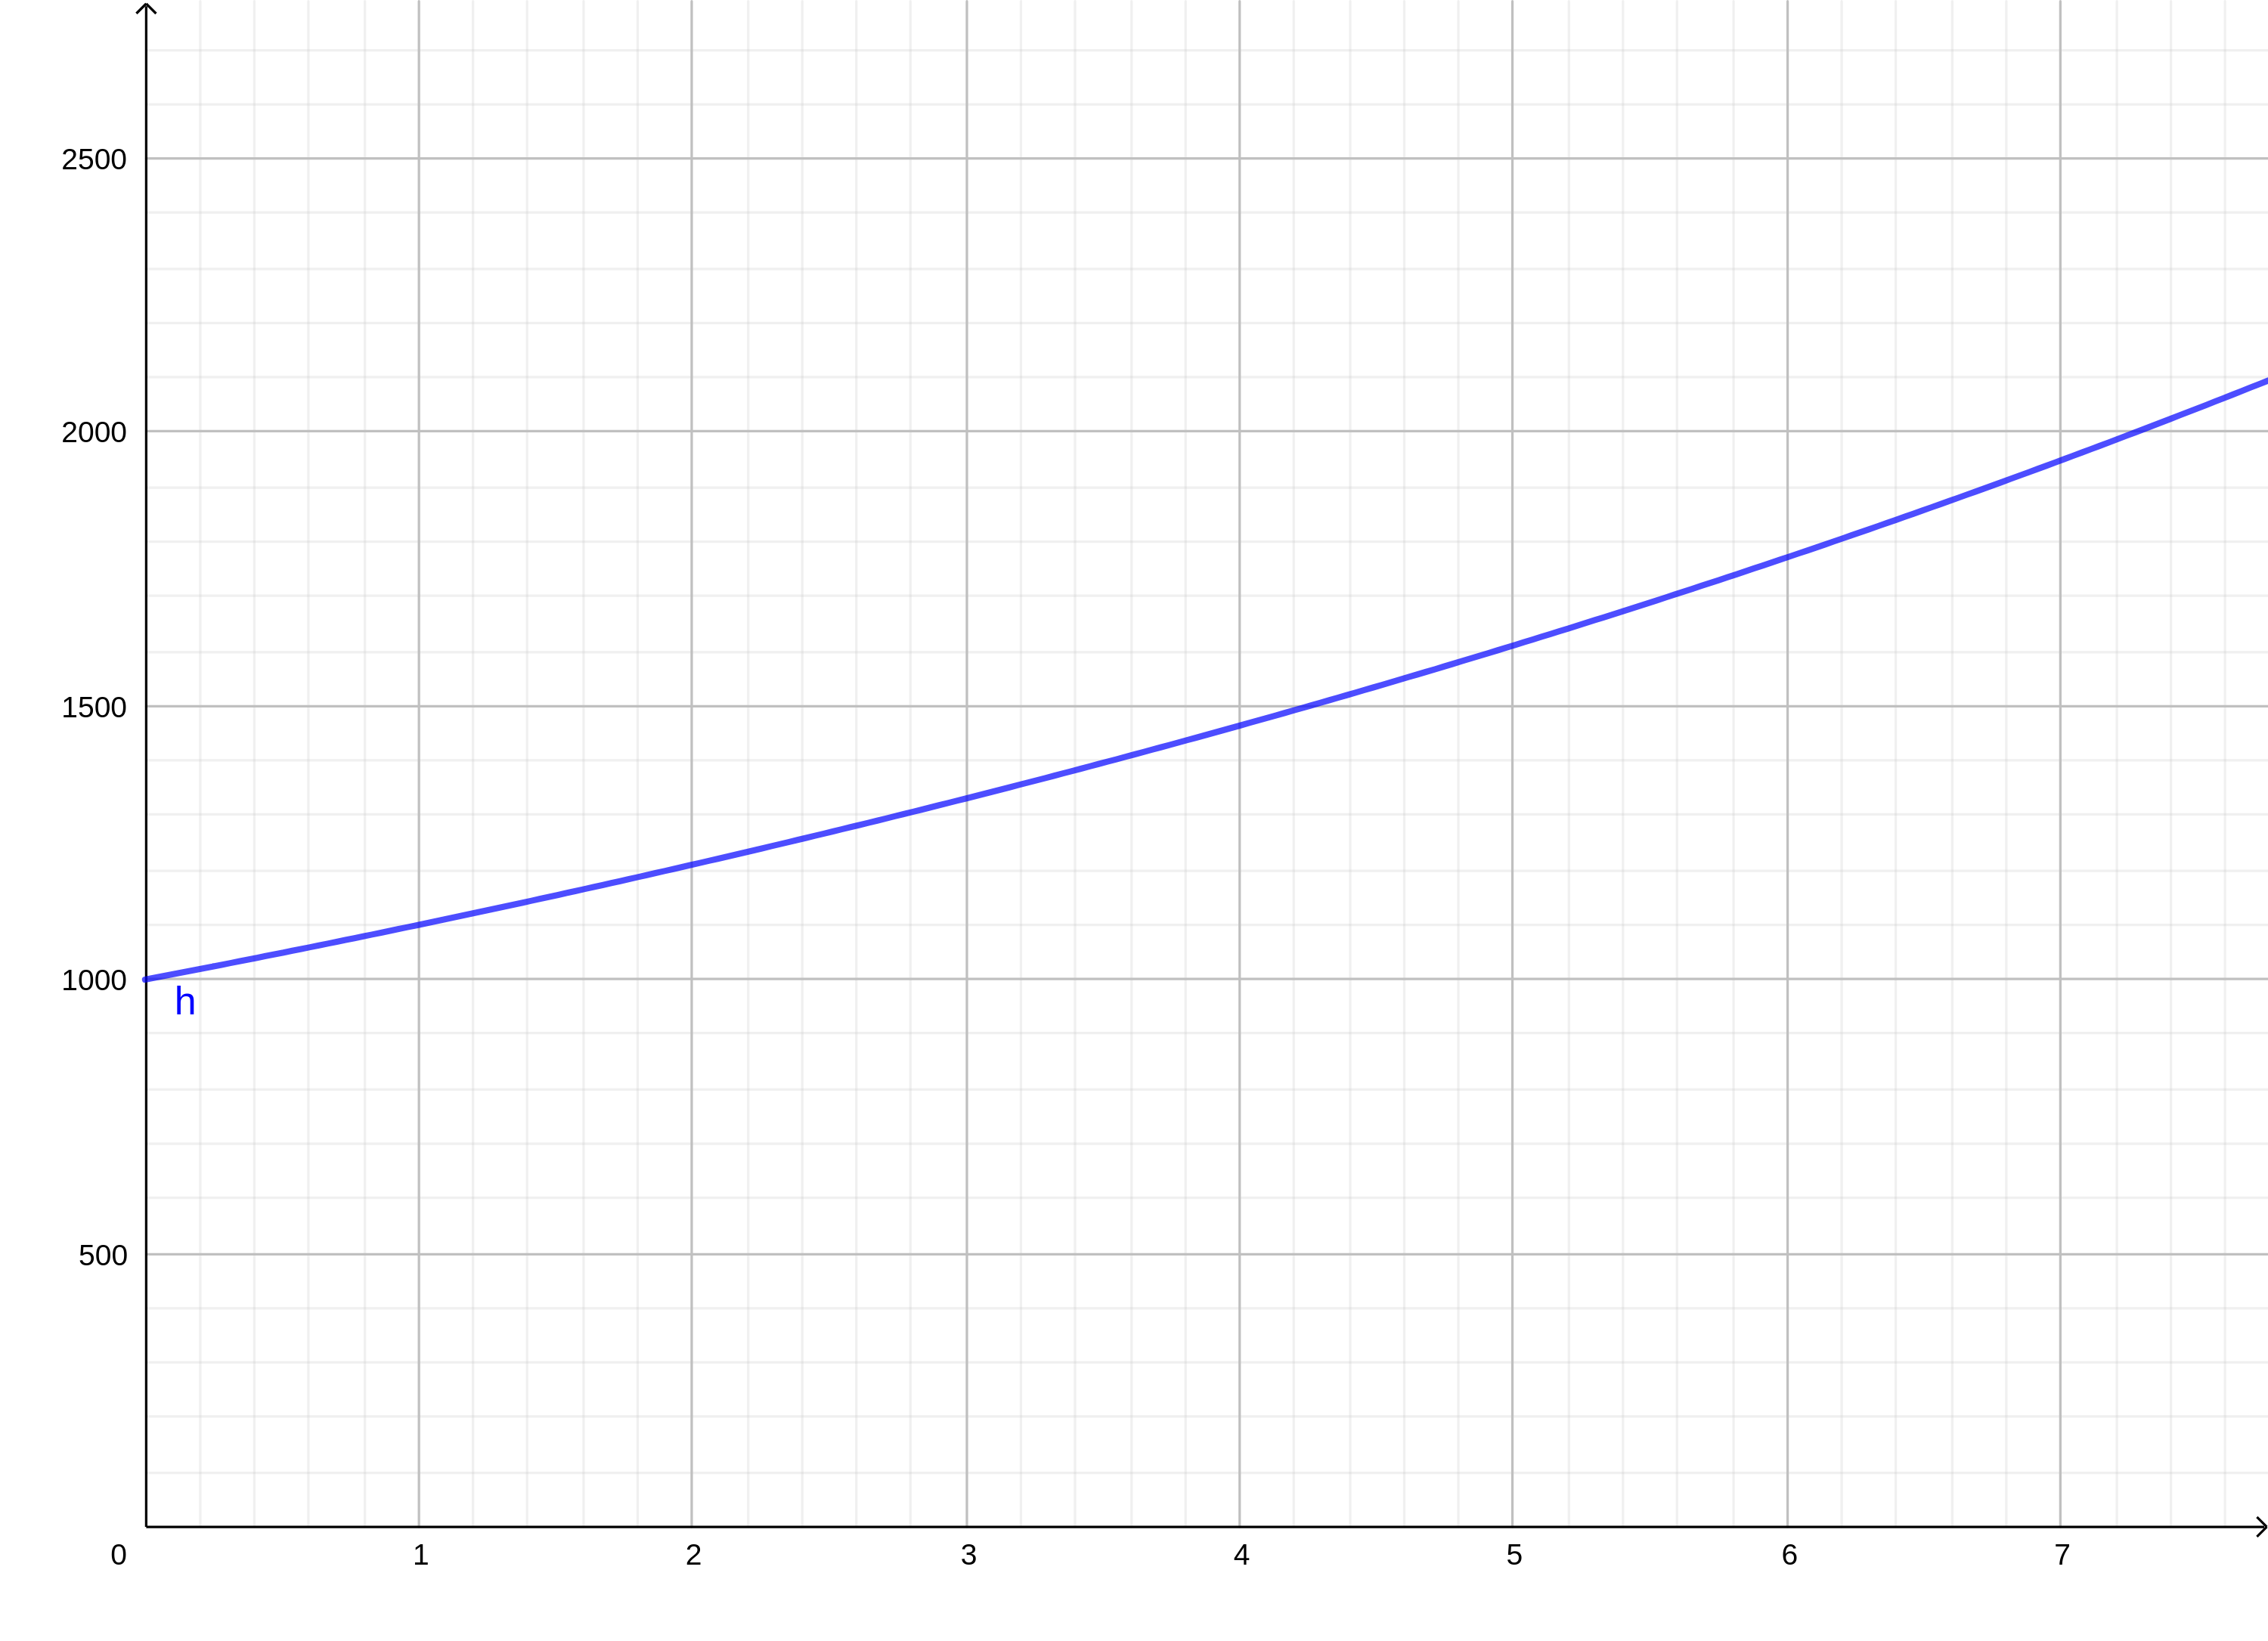
\includegraphics[height=4cm]{./images/Q2-resposta.png}
      \part[1.5]  Quando o montante é $R\$ 2000$?
      $1000 \cdot 1,1^x = 2000 = 2 \cdot 1000$ \\
      $1,1^x = 2 $, dividindo por $1000$ em ambos os lados.\\
      $\log 1,1^x = \log 2 $ \\
      $x \cdot \log 1,1 = \log 2 $ \\
      $x  = \frac{\log 2}{\log 1,1} $ \\
      $x \approx 0,3/0,04 = 7,5$, ou seja, 7 anos e meio aproximadamente.
    \end{parts}

    \question Um determinado programa de computador inicia seu processo com $1MiB$ de memória RAM.
    Sabe-se que sempre que ele precisa de mais memória ele requisita (ao Sistema Operacional) 
    a quantidade de memória que tem no momento da requisição. Por exemplo, se ele tem $3MiB$
    de memória e necessita de mais, ele requisita mais $3MiB$, ficando com $6MiB$ (donde $3MiB$ estão ocupados e $3MiB$ livres).
    José, identifica que o programa está usando $50MiB$.
    \begin{parts}
        \part[1.5] Quantas vezes o programa solicitou memória ao Sistema Operacional?
        Como o programa está usando $50MiB$ ele tem que ter requisitado memória até chegar a este valor ou ultrapassar.
        Como a cada requisição ele dobra a quantidade de memória que tem acesso, temos: \\
        Início: $1MiB$ \\
        1ª req: $2MiB$ \\
        2ª req: $4MiB$ \\
        3ª req: $8MiB$ \\
        4ª req: $16MiB$ \\
        5ª req: $32MiB$ \\
        6ª req: $64MiB$ \\
        Portanto o programa solicitou memória 6 vezes.
    \end{parts}
        \question Seja $f(x) = 3^{5x}$ e $g(x) = 3^x$, calcule:
        \begin{parts}
            \part[0.5] $(f(x))^2$ \\
            $f(x) \cdot f(x) = 3^{5x} \cdot 3^{5x} = 3^{5x+5x} = 3^{10x}$ ou ainda, \\
            $f(x) \cdot f(x) = (3^{5x})^2 = 3^{5x \cdot 2} = 3^{10x}$ \\
            \part[0.5] $\dfrac{f(x)}{g(x)}$ \\
            $\dfrac{f(x)}{g(x)} = \dfrac{3^{5x}}{3^x} = 3^{5x - x} = 3^{4x}$

        \end{parts}
\end{questions}
Formulário:  \\
\begin{align*}
    \log 2 \approx 0,3 &&
    \log 1,1 \approx 0,04 &&
    \log x^k = k \cdot \log x \\
    \frac{\log a}{\log b} = \log_b a &&
    \log_c {(a\cdot b)} = \log_c a + \log_c b &&
    \log_c \frac{a}{b} = \log_c a - \log_c b
\end{align*}
\end{document}
